% Options for packages loaded elsewhere
\PassOptionsToPackage{unicode}{hyperref}
\PassOptionsToPackage{hyphens}{url}
%
\documentclass[
  12pt,
  a4paper,
]{article}
\usepackage{amsmath,amssymb}
\usepackage{lmodern}
\usepackage{iftex}
\ifPDFTeX
  \usepackage[T1]{fontenc}
  \usepackage[utf8]{inputenc}
  \usepackage{textcomp} % provide euro and other symbols
\else % if luatex or xetex
  \usepackage{unicode-math}
  \defaultfontfeatures{Scale=MatchLowercase}
  \defaultfontfeatures[\rmfamily]{Ligatures=TeX,Scale=1}
\fi
% Use upquote if available, for straight quotes in verbatim environments
\IfFileExists{upquote.sty}{\usepackage{upquote}}{}
\IfFileExists{microtype.sty}{% use microtype if available
  \usepackage[]{microtype}
  \UseMicrotypeSet[protrusion]{basicmath} % disable protrusion for tt fonts
}{}
\makeatletter
\@ifundefined{KOMAClassName}{% if non-KOMA class
  \IfFileExists{parskip.sty}{%
    \usepackage{parskip}
  }{% else
    \setlength{\parindent}{0pt}
    \setlength{\parskip}{6pt plus 2pt minus 1pt}}
}{% if KOMA class
  \KOMAoptions{parskip=half}}
\makeatother
\usepackage{xcolor}
\IfFileExists{xurl.sty}{\usepackage{xurl}}{} % add URL line breaks if available
\IfFileExists{bookmark.sty}{\usepackage{bookmark}}{\usepackage{hyperref}}
\hypersetup{
  hidelinks,
  pdfcreator={LaTeX via pandoc}}
\urlstyle{same} % disable monospaced font for URLs
\usepackage{color}
\usepackage{fancyvrb}
\newcommand{\VerbBar}{|}
\newcommand{\VERB}{\Verb[commandchars=\\\{\}]}
\DefineVerbatimEnvironment{Highlighting}{Verbatim}{commandchars=\\\{\}}
% Add ',fontsize=\small' for more characters per line
\newenvironment{Shaded}{}{}
\newcommand{\AlertTok}[1]{\textcolor[rgb]{1.00,0.00,0.00}{\textbf{#1}}}
\newcommand{\AnnotationTok}[1]{\textcolor[rgb]{0.38,0.63,0.69}{\textbf{\textit{#1}}}}
\newcommand{\AttributeTok}[1]{\textcolor[rgb]{0.49,0.56,0.16}{#1}}
\newcommand{\BaseNTok}[1]{\textcolor[rgb]{0.25,0.63,0.44}{#1}}
\newcommand{\BuiltInTok}[1]{#1}
\newcommand{\CharTok}[1]{\textcolor[rgb]{0.25,0.44,0.63}{#1}}
\newcommand{\CommentTok}[1]{\textcolor[rgb]{0.38,0.63,0.69}{\textit{#1}}}
\newcommand{\CommentVarTok}[1]{\textcolor[rgb]{0.38,0.63,0.69}{\textbf{\textit{#1}}}}
\newcommand{\ConstantTok}[1]{\textcolor[rgb]{0.53,0.00,0.00}{#1}}
\newcommand{\ControlFlowTok}[1]{\textcolor[rgb]{0.00,0.44,0.13}{\textbf{#1}}}
\newcommand{\DataTypeTok}[1]{\textcolor[rgb]{0.56,0.13,0.00}{#1}}
\newcommand{\DecValTok}[1]{\textcolor[rgb]{0.25,0.63,0.44}{#1}}
\newcommand{\DocumentationTok}[1]{\textcolor[rgb]{0.73,0.13,0.13}{\textit{#1}}}
\newcommand{\ErrorTok}[1]{\textcolor[rgb]{1.00,0.00,0.00}{\textbf{#1}}}
\newcommand{\ExtensionTok}[1]{#1}
\newcommand{\FloatTok}[1]{\textcolor[rgb]{0.25,0.63,0.44}{#1}}
\newcommand{\FunctionTok}[1]{\textcolor[rgb]{0.02,0.16,0.49}{#1}}
\newcommand{\ImportTok}[1]{#1}
\newcommand{\InformationTok}[1]{\textcolor[rgb]{0.38,0.63,0.69}{\textbf{\textit{#1}}}}
\newcommand{\KeywordTok}[1]{\textcolor[rgb]{0.00,0.44,0.13}{\textbf{#1}}}
\newcommand{\NormalTok}[1]{#1}
\newcommand{\OperatorTok}[1]{\textcolor[rgb]{0.40,0.40,0.40}{#1}}
\newcommand{\OtherTok}[1]{\textcolor[rgb]{0.00,0.44,0.13}{#1}}
\newcommand{\PreprocessorTok}[1]{\textcolor[rgb]{0.74,0.48,0.00}{#1}}
\newcommand{\RegionMarkerTok}[1]{#1}
\newcommand{\SpecialCharTok}[1]{\textcolor[rgb]{0.25,0.44,0.63}{#1}}
\newcommand{\SpecialStringTok}[1]{\textcolor[rgb]{0.73,0.40,0.53}{#1}}
\newcommand{\StringTok}[1]{\textcolor[rgb]{0.25,0.44,0.63}{#1}}
\newcommand{\VariableTok}[1]{\textcolor[rgb]{0.10,0.09,0.49}{#1}}
\newcommand{\VerbatimStringTok}[1]{\textcolor[rgb]{0.25,0.44,0.63}{#1}}
\newcommand{\WarningTok}[1]{\textcolor[rgb]{0.38,0.63,0.69}{\textbf{\textit{#1}}}}
\usepackage{longtable,booktabs,array}
\usepackage{calc} % for calculating minipage widths
% Correct order of tables after \paragraph or \subparagraph
\usepackage{etoolbox}
\makeatletter
\patchcmd\longtable{\par}{\if@noskipsec\mbox{}\fi\par}{}{}
\makeatother
% Allow footnotes in longtable head/foot
\IfFileExists{footnotehyper.sty}{\usepackage{footnotehyper}}{\usepackage{footnote}}
\makesavenoteenv{longtable}
\setlength{\emergencystretch}{3em} % prevent overfull lines
\providecommand{\tightlist}{%
  \setlength{\itemsep}{0pt}\setlength{\parskip}{0pt}}
\setcounter{secnumdepth}{-\maxdimen} % remove section numbering
\ifLuaTeX
  \usepackage{selnolig}  % disable illegal ligatures
\fi

\newcommand{\thetitle}{Реализация модели вселенной. Трехмерная визуализация.
Модель Солнце-Земля}
\newcommand{\theauthor}{Старовойтов А. И.}
\newcommand{\theteacher}{Посевин Д. П.}
\newcommand{\thegroup}{ИУ9-21Б}
\newcommand{\thecourse}{Языки и методы программирования}
\newcommand{\thenumber}{2.2}

\usepackage{graphicx}
\usepackage{geometry}

\usepackage{fontspec}
\setmainfont{DejaVu Serif}
\setsansfont{DejaVu Sans}
\setmonofont{DejaVu Sans Mono}
\defaultfontfeatures{Ligatures=TeX}
\usepackage{polyglossia}
\usepackage[autostyle=true]{csquotes}
\setdefaultlanguage{russian}
\setotherlanguage{english}

\usepackage{fvextra}

\renewcommand{\maketitle}
{
\newgeometry{
  left=0.7in,
  right=0.7in,
}
\begin{titlepage}
    \centering
    Федеральное государственное бюджетное образовательное учреждение\\
    высшего профессионального образования\\
    <<Московский государственный технический университет\\
    имени Н.Э. Баумана>>\\
    (МГТУ им. Н.Э. Баумана)
    \vspace{1cm}

    \flushleft

    Факультет: \underline{Информатика и системы управления}\\
    Кафедра: \underline{Теоретическая информатика и компьютерные технологии}

    \centering
    \topskip0pt
    \vspace*{\fill}
    Лабораторная работа №\thenumber{}\\
    <<\thetitle{}>>\\
    по курсу: <<\thecourse{}>>
    \vspace*{\fill}
    \centering

    %\vspace{2cm}

    \hfill\begin{minipage}{0.4\linewidth}
        Выполнил:\\
        Студент группы \thegroup{}\\
        \theauthor\\
        \\
        Проверил:\\
        \theteacher
    \end{minipage}

    \vfill

    Москва, \the\year{}

\end{titlepage}
\restoregeometry{}
}

\usepackage{fvextra}
\DefineVerbatimEnvironment{Highlighting}{Verbatim}{breaklines,commandchars=\\\{\}}

\begin{document}
\maketitle

\hypertarget{ux446ux435ux43bux438}{%
\section{Цели}\label{ux446ux435ux43bux438}}

Реализовать модель вселенной. Каждый элемент вселенной должен быть
объектом некоего публичного класса, который инициализируется
вспомогательным публичным классом порождающим эту вселенную. При
инициализации экземпляров класса частиц моделируемой вселенной
необходимо подсчитывать количество частиц вселенной используя статичное
экземплярное поле защищенное от изменения из объектов внешних классов
путем реализации статичного метода. Сформировать исходные данные и
определить необходимые экземплярные поля для хранения состояния объектов
частиц вселенной в соответствии с условием задачи и реализовать расчет.

Моделировать движение материальных точек под действием силы
гравитационного взаимодействия. Полученные данные визуализировать в виде
трехмерного графика с помощью \texttt{gnuplot}.

\hypertarget{ux437ux430ux434ux430ux447ux438}{%
\section{Задачи}\label{ux437ux430ux434ux430ux447ux438}}

Расчет траекторий материальных точек вселенных и их визуализация с
использованием \texttt{gnuplot}. Построение модели Солнце--Земля.

\hypertarget{ux440ux435ux448ux435ux43dux438ux435}{%
\section{Решение}\label{ux440ux435ux448ux435ux43dux438ux435}}

\hypertarget{test.java}{%
\subsection{\texorpdfstring{\texttt{Test.java}}{Test.java}}\label{test.java}}

Объявим класс для тестирования:

\begin{Shaded}
\begin{Highlighting}[]
\KeywordTok{public} \KeywordTok{class}\NormalTok{ test }\OperatorTok{\{}
    \KeywordTok{public} \DataTypeTok{static} \DataTypeTok{void} \FunctionTok{main}\OperatorTok{(}\NormalTok{string}\OperatorTok{[]}\NormalTok{ args}\OperatorTok{)} \OperatorTok{\{}
\end{Highlighting}
\end{Shaded}

Создадим новую вселенную:

\begin{Shaded}
\begin{Highlighting}[]
\NormalTok{Universe universe }\OperatorTok{=} \KeywordTok{new} \FunctionTok{Universe}\OperatorTok{();}
\end{Highlighting}
\end{Shaded}

Добавим в эту вселенную материальную точку --- модель Солнца:

\begin{longtable}[]{@{}lll@{}}
\toprule
Начальные координаты, м & Начальная скорость, м/с & Масса, кг \\
\midrule
\endhead
\((0, 0, 0)\) & \((0, 0, 0)\) & \(1,9885*10^{30}\) \\
\bottomrule
\end{longtable}

\begin{Shaded}
\begin{Highlighting}[]
\NormalTok{universe}\OperatorTok{.}\FunctionTok{add}\OperatorTok{(}\DecValTok{0}\OperatorTok{,} \DecValTok{0}\OperatorTok{,} \DecValTok{0}\OperatorTok{,} \DecValTok{0}\OperatorTok{,} \DecValTok{0}\OperatorTok{,} \DecValTok{0}\OperatorTok{,} \FloatTok{1.989e30}\OperatorTok{);} \CommentTok{// солнце}
\end{Highlighting}
\end{Shaded}

И модель Земли:

\begin{longtable}[]{@{}lll@{}}
\toprule
Начальные координаты, м & Начальная скорость, м/с & Масса, кг \\
\midrule
\endhead
\((147098290*10^3, 0, 0)\) & \((0, 30270, 0)\) & \(5,9726*10^{24}\) \\
\bottomrule
\end{longtable}

\begin{Shaded}
\begin{Highlighting}[]
\NormalTok{universe}\OperatorTok{.}\FunctionTok{add}\OperatorTok{(}\FloatTok{147098290e3}\OperatorTok{,} \DecValTok{0}\OperatorTok{,} \DecValTok{0}\OperatorTok{,} \DecValTok{0}\OperatorTok{,} \DecValTok{30270}\OperatorTok{,} \DecValTok{0}\OperatorTok{,} \FloatTok{5.972e24}\OperatorTok{);} \CommentTok{// земля}
\end{Highlighting}
\end{Shaded}

Далее, построим траектории движения планет за 1 год и запишем в файл:

\begin{Shaded}
\begin{Highlighting}[]
\NormalTok{        universe}\OperatorTok{.}\FunctionTok{dump}\OperatorTok{(}\StringTok{"plot.dat"}\OperatorTok{,} \KeywordTok{false}\OperatorTok{);}
        \ControlFlowTok{for} \OperatorTok{(}\DataTypeTok{int}\NormalTok{ i }\OperatorTok{=} \DecValTok{0}\OperatorTok{;}\NormalTok{ i }\OperatorTok{\textless{}} \DecValTok{1}\OperatorTok{*}\DecValTok{24}\OperatorTok{*}\DecValTok{365}\OperatorTok{;} \OperatorTok{++}\NormalTok{i}\OperatorTok{)} \OperatorTok{\{} \CommentTok{// год}
\NormalTok{            universe}\OperatorTok{.}\FunctionTok{recalcCoords}\OperatorTok{(}\DecValTok{60}\OperatorTok{*}\DecValTok{60}\OperatorTok{);} \CommentTok{// час}
\NormalTok{            universe}\OperatorTok{.}\FunctionTok{dump}\OperatorTok{(}\StringTok{"plot.dat"}\OperatorTok{,} \KeywordTok{true}\OperatorTok{);}
        \OperatorTok{\}}
    \OperatorTok{\}}
\OperatorTok{\};}
\end{Highlighting}
\end{Shaded}

Метод \texttt{recalcCoords} \((\Delta t)\) обновляет координаты
материальных точек вселенной спустя \(\Delta t\).

\hypertarget{universe.java}{%
\subsection{\texorpdfstring{\texttt{Universe.java}}{Universe.java}}\label{universe.java}}

Импорт необходимых пакетов и объявление класса Вселенной:

\begin{Shaded}
\begin{Highlighting}[]
\KeywordTok{import} \ImportTok{java}\OperatorTok{.}\ImportTok{util}\OperatorTok{.}\ImportTok{Random}\OperatorTok{;}
\KeywordTok{import} \ImportTok{java}\OperatorTok{.}\ImportTok{io}\OperatorTok{.*;}
\KeywordTok{import} \ImportTok{java}\OperatorTok{.}\ImportTok{lang}\OperatorTok{.}\ImportTok{Math}\OperatorTok{;}
\KeywordTok{import} \ImportTok{java}\OperatorTok{.}\ImportTok{util}\OperatorTok{.}\ImportTok{ArrayList}\OperatorTok{;}

\KeywordTok{public} \KeywordTok{class}\NormalTok{ Universe }\OperatorTok{\{}
\end{Highlighting}
\end{Shaded}

Объявим вспомогательный класс \texttt{Point}, реализующий геометрическую
точку.

\begin{Shaded}
\begin{Highlighting}[]
\KeywordTok{public} \KeywordTok{class} \BuiltInTok{Point} \OperatorTok{\{}
    \KeywordTok{private} \DataTypeTok{double}\NormalTok{ x}\OperatorTok{;}
    \KeywordTok{private} \DataTypeTok{double}\NormalTok{ y}\OperatorTok{;}
    \KeywordTok{private} \DataTypeTok{double}\NormalTok{ z}\OperatorTok{;}

    \KeywordTok{public} \BuiltInTok{Point}\OperatorTok{(}\DataTypeTok{double}\NormalTok{ x}\OperatorTok{,} \DataTypeTok{double}\NormalTok{ y}\OperatorTok{,} \DataTypeTok{double}\NormalTok{ z}\OperatorTok{)} \OperatorTok{\{}
        \KeywordTok{this}\OperatorTok{.}\FunctionTok{x} \OperatorTok{=}\NormalTok{ x}\OperatorTok{;}
        \KeywordTok{this}\OperatorTok{.}\FunctionTok{y} \OperatorTok{=}\NormalTok{ y}\OperatorTok{;}
        \KeywordTok{this}\OperatorTok{.}\FunctionTok{z} \OperatorTok{=}\NormalTok{ z}\OperatorTok{;}
    \OperatorTok{\}}

    \KeywordTok{public} \DataTypeTok{double} \FunctionTok{calcDist}\OperatorTok{(}\BuiltInTok{Point}\NormalTok{ p}\OperatorTok{)} \OperatorTok{\{}
        \ControlFlowTok{return} \BuiltInTok{Math}\OperatorTok{.}\FunctionTok{sqrt}\OperatorTok{(}\BuiltInTok{Math}\OperatorTok{.}\FunctionTok{pow}\OperatorTok{(}\KeywordTok{this}\OperatorTok{.}\FunctionTok{x} \OperatorTok{{-}}\NormalTok{ p}\OperatorTok{.}\FunctionTok{x}\OperatorTok{,} \DecValTok{2}\OperatorTok{)}
                         \OperatorTok{+} \BuiltInTok{Math}\OperatorTok{.}\FunctionTok{pow}\OperatorTok{(}\KeywordTok{this}\OperatorTok{.}\FunctionTok{y} \OperatorTok{{-}}\NormalTok{ p}\OperatorTok{.}\FunctionTok{y}\OperatorTok{,} \DecValTok{2}\OperatorTok{)}
                         \OperatorTok{+} \BuiltInTok{Math}\OperatorTok{.}\FunctionTok{pow}\OperatorTok{(}\KeywordTok{this}\OperatorTok{.}\FunctionTok{z} \OperatorTok{{-}}\NormalTok{ p}\OperatorTok{.}\FunctionTok{z}\OperatorTok{,} \DecValTok{2}\OperatorTok{));}
    \OperatorTok{\}}

    \KeywordTok{public} \BuiltInTok{String} \FunctionTok{toString}\OperatorTok{()} \OperatorTok{\{}
        \ControlFlowTok{return}\NormalTok{ x }\OperatorTok{+} \StringTok{" "} \OperatorTok{+}\NormalTok{ y }\OperatorTok{+} \StringTok{" "} \OperatorTok{+}\NormalTok{ z}\OperatorTok{;}
    \OperatorTok{\}}

    \KeywordTok{public} \DataTypeTok{double} \FunctionTok{getR}\OperatorTok{()} \OperatorTok{\{}
        \ControlFlowTok{return} \BuiltInTok{Math}\OperatorTok{.}\FunctionTok{sqrt}\OperatorTok{(}\BuiltInTok{Math}\OperatorTok{.}\FunctionTok{pow}\OperatorTok{(}\KeywordTok{this}\OperatorTok{.}\FunctionTok{x}\OperatorTok{,} \DecValTok{2}\OperatorTok{)}
                         \OperatorTok{+} \BuiltInTok{Math}\OperatorTok{.}\FunctionTok{pow}\OperatorTok{(}\KeywordTok{this}\OperatorTok{.}\FunctionTok{y}\OperatorTok{,} \DecValTok{2}\OperatorTok{)}
                         \OperatorTok{+} \BuiltInTok{Math}\OperatorTok{.}\FunctionTok{pow}\OperatorTok{(}\KeywordTok{this}\OperatorTok{.}\FunctionTok{z}\OperatorTok{,} \DecValTok{2}\OperatorTok{));}
    \OperatorTok{\}}

    \KeywordTok{public} \DataTypeTok{void} \FunctionTok{add}\OperatorTok{(}\BuiltInTok{Point}\NormalTok{ p}\OperatorTok{)} \OperatorTok{\{}
        \KeywordTok{this}\OperatorTok{.}\FunctionTok{x} \OperatorTok{+=}\NormalTok{ p}\OperatorTok{.}\FunctionTok{x}\OperatorTok{;}
        \KeywordTok{this}\OperatorTok{.}\FunctionTok{y} \OperatorTok{+=}\NormalTok{ p}\OperatorTok{.}\FunctionTok{y}\OperatorTok{;}
        \KeywordTok{this}\OperatorTok{.}\FunctionTok{z} \OperatorTok{+=}\NormalTok{ p}\OperatorTok{.}\FunctionTok{z}\OperatorTok{;}
    \OperatorTok{\}}

    \KeywordTok{public} \DataTypeTok{void} \FunctionTok{mult}\OperatorTok{(}\DataTypeTok{double}\NormalTok{ m}\OperatorTok{)} \OperatorTok{\{}
        \KeywordTok{this}\OperatorTok{.}\FunctionTok{x} \OperatorTok{*=}\NormalTok{ m}\OperatorTok{;}
        \KeywordTok{this}\OperatorTok{.}\FunctionTok{y} \OperatorTok{*=}\NormalTok{ m}\OperatorTok{;}
        \KeywordTok{this}\OperatorTok{.}\FunctionTok{z} \OperatorTok{*=}\NormalTok{ m}\OperatorTok{;}
    \OperatorTok{\}}
\OperatorTok{\}}
\end{Highlighting}
\end{Shaded}

Далее, объявим класс \texttt{Particle}, реализующий частицу:

\begin{Shaded}
\begin{Highlighting}[]
\KeywordTok{public} \KeywordTok{class}\NormalTok{ Particle }\OperatorTok{\{}
    \KeywordTok{private} \DataTypeTok{double}\NormalTok{ m}\OperatorTok{;}
    \KeywordTok{private} \BuiltInTok{Point}\NormalTok{ pos}\OperatorTok{;}
    \KeywordTok{private} \BuiltInTok{Point}\NormalTok{ v}\OperatorTok{;}
\end{Highlighting}
\end{Shaded}

Поля класса: масса, координаты, вектор скорости.

Будем хранить точки всех вселенных в списке \texttt{particles}. Это
необходимо для расчета силы гравитационного взаимодействия в случае
нескольких Вселенных.

\begin{Shaded}
\begin{Highlighting}[]
\KeywordTok{private} \DataTypeTok{static} \BuiltInTok{ArrayList}\OperatorTok{\textless{}}\NormalTok{Particle}\OperatorTok{\textgreater{}}\NormalTok{ particles }\OperatorTok{=} \KeywordTok{new} \BuiltInTok{ArrayList}\OperatorTok{\textless{}}\NormalTok{Particle}\OperatorTok{\textgreater{}();}
\end{Highlighting}
\end{Shaded}

Объявим конструктор:

\begin{Shaded}
\begin{Highlighting}[]
\KeywordTok{public} \FunctionTok{Particle}\OperatorTok{(}\DataTypeTok{double}\NormalTok{ x}\OperatorTok{,} \DataTypeTok{double}\NormalTok{ y}\OperatorTok{,} \DataTypeTok{double}\NormalTok{ z}\OperatorTok{,} \DataTypeTok{double}\NormalTok{ vx}\OperatorTok{,} \DataTypeTok{double}\NormalTok{ vy}\OperatorTok{,} \DataTypeTok{double}\NormalTok{ vz}\OperatorTok{,} \DataTypeTok{double}\NormalTok{ m}\OperatorTok{)} \OperatorTok{\{}
    \KeywordTok{this}\OperatorTok{.}\FunctionTok{pos} \OperatorTok{=} \KeywordTok{new} \BuiltInTok{Point}\OperatorTok{(}\NormalTok{x}\OperatorTok{,}\NormalTok{ y}\OperatorTok{,}\NormalTok{ z}\OperatorTok{);}
    \KeywordTok{this}\OperatorTok{.}\FunctionTok{v} \OperatorTok{=} \KeywordTok{new} \BuiltInTok{Point}\OperatorTok{(}\NormalTok{vx}\OperatorTok{,}\NormalTok{ vy}\OperatorTok{,}\NormalTok{ vz}\OperatorTok{);}
    \KeywordTok{this}\OperatorTok{.}\FunctionTok{m} \OperatorTok{=}\NormalTok{ m}\OperatorTok{;}
\NormalTok{    particles}\OperatorTok{.}\FunctionTok{add}\OperatorTok{(}\KeywordTok{this}\OperatorTok{);}
\OperatorTok{\}}
\end{Highlighting}
\end{Shaded}

Функция преобразования к строковому типу:

\begin{Shaded}
\begin{Highlighting}[]
\AttributeTok{@Override}
\KeywordTok{public} \BuiltInTok{String} \FunctionTok{toString}\OperatorTok{()} \OperatorTok{\{}
    \ControlFlowTok{return}\NormalTok{ m }\OperatorTok{+} \StringTok{" "} \OperatorTok{+}\NormalTok{ pos }\OperatorTok{+} \StringTok{" "} \OperatorTok{+}\NormalTok{ v}\OperatorTok{;}
\OperatorTok{\}}
\end{Highlighting}
\end{Shaded}

Метод для пересчета координат всех точек спустя \(\Delta t\):

\begin{Shaded}
\begin{Highlighting}[]
\KeywordTok{public} \DataTypeTok{static} \DataTypeTok{void} \FunctionTok{recalcAllCoords}\OperatorTok{(}\DataTypeTok{double}\NormalTok{ time}\OperatorTok{)} \OperatorTok{\{}
\end{Highlighting}
\end{Shaded}

Считаем вектор равнодействующей силам гравитационного взаимодействия для
каждой точки:

\begin{Shaded}
\begin{Highlighting}[]
\BuiltInTok{Point}\OperatorTok{[]}\NormalTok{ forces }\OperatorTok{=} \KeywordTok{new} \BuiltInTok{Point}\OperatorTok{[}\NormalTok{particles}\OperatorTok{.}\FunctionTok{size}\OperatorTok{()];}
\ControlFlowTok{for} \OperatorTok{(}\DataTypeTok{int}\NormalTok{ i }\OperatorTok{=} \DecValTok{0}\OperatorTok{;}\NormalTok{ i }\OperatorTok{\textless{}}\NormalTok{ particles}\OperatorTok{.}\FunctionTok{size}\OperatorTok{();} \OperatorTok{++}\NormalTok{i}\OperatorTok{)} \OperatorTok{\{}
\NormalTok{    forces}\OperatorTok{[}\NormalTok{i}\OperatorTok{]} \OperatorTok{=}\NormalTok{ particles}\OperatorTok{.}\FunctionTok{get}\OperatorTok{(}\NormalTok{i}\OperatorTok{).}\FunctionTok{calcOverallF}\OperatorTok{();}
\OperatorTok{\}}
\end{Highlighting}
\end{Shaded}

С учетом времени и равнодействующей силы обновляем координаты каждой
точки:

\begin{Shaded}
\begin{Highlighting}[]
    \ControlFlowTok{for} \OperatorTok{(}\DataTypeTok{int}\NormalTok{ i }\OperatorTok{=} \DecValTok{0}\OperatorTok{;}\NormalTok{ i }\OperatorTok{\textless{}}\NormalTok{ particles}\OperatorTok{.}\FunctionTok{size}\OperatorTok{();} \OperatorTok{++}\NormalTok{i}\OperatorTok{)} \OperatorTok{\{}
\NormalTok{        particles}\OperatorTok{.}\FunctionTok{get}\OperatorTok{(}\NormalTok{i}\OperatorTok{).}\FunctionTok{recalcCoords}\OperatorTok{(}\NormalTok{time}\OperatorTok{,}\NormalTok{ forces}\OperatorTok{[}\NormalTok{i}\OperatorTok{]);}
    \OperatorTok{\}}
\OperatorTok{\}}
\end{Highlighting}
\end{Shaded}

Метод для нахождения силы гравитационного взаимодействия, оказываемой
одной точкой на другую:

\begin{Shaded}
\begin{Highlighting}[]
\KeywordTok{private} \BuiltInTok{Point} \FunctionTok{calcF}\OperatorTok{(}\NormalTok{Particle p}\OperatorTok{)} \OperatorTok{\{}
\end{Highlighting}
\end{Shaded}

Гравитационная постоянная:
\(G = 6,67430*10^{-11} \text{м}^{3}*\text{кг}^{-1}*\text{с}^{-2}\).

\begin{Shaded}
\begin{Highlighting}[]
\DataTypeTok{final} \DataTypeTok{double}\NormalTok{ G }\OperatorTok{=} \FloatTok{6.67430e{-}11}\OperatorTok{;}
\end{Highlighting}
\end{Shaded}

Считаем расстояние между точками:

\begin{Shaded}
\begin{Highlighting}[]
\DataTypeTok{double}\NormalTok{ r }\OperatorTok{=} \KeywordTok{this}\OperatorTok{.}\FunctionTok{pos}\OperatorTok{.}\FunctionTok{calcDist}\OperatorTok{(}\NormalTok{p}\OperatorTok{.}\FunctionTok{pos}\OperatorTok{);}
\end{Highlighting}
\end{Shaded}

И, наконец, модуль силы гравитационного взаимодействия:

\begin{equation*}
|F| = G*\frac{m_{1} * m_{2}}{r^{2}}
\end{equation*}

\begin{Shaded}
\begin{Highlighting}[]
\DataTypeTok{double}\NormalTok{ modF }\OperatorTok{=}\NormalTok{ G }\OperatorTok{*} \KeywordTok{this}\OperatorTok{.}\FunctionTok{m} \OperatorTok{*}\NormalTok{ p}\OperatorTok{.}\FunctionTok{m} \OperatorTok{/} \OperatorTok{(}\NormalTok{r}\OperatorTok{*}\NormalTok{r}\OperatorTok{);}
\end{Highlighting}
\end{Shaded}

Теперь можем найти вектор силы. Для этого вектор из одной точки в
другую, домножим на отношение модуля силы и длины этого вектора:

\begin{equation*}
F = \frac{|F|}{|\vec{AB}|}\vec{AB}
\end{equation*}

\begin{Shaded}
\begin{Highlighting}[]
    \BuiltInTok{Point}\NormalTok{ F }\OperatorTok{=} \KeywordTok{new} \BuiltInTok{Point}\OperatorTok{(}\NormalTok{p}\OperatorTok{.}\FunctionTok{pos}\OperatorTok{.}\FunctionTok{x} \OperatorTok{{-}} \KeywordTok{this}\OperatorTok{.}\FunctionTok{pos}\OperatorTok{.}\FunctionTok{x}\OperatorTok{,}
\NormalTok{                        p}\OperatorTok{.}\FunctionTok{pos}\OperatorTok{.}\FunctionTok{y} \OperatorTok{{-}} \KeywordTok{this}\OperatorTok{.}\FunctionTok{pos}\OperatorTok{.}\FunctionTok{y}\OperatorTok{,}
\NormalTok{                        p}\OperatorTok{.}\FunctionTok{pos}\OperatorTok{.}\FunctionTok{z} \OperatorTok{{-}} \KeywordTok{this}\OperatorTok{.}\FunctionTok{pos}\OperatorTok{.}\FunctionTok{z}\OperatorTok{);}
\NormalTok{    F}\OperatorTok{.}\FunctionTok{mult}\OperatorTok{(}\NormalTok{modF }\OperatorTok{/}\NormalTok{ F}\OperatorTok{.}\FunctionTok{getR}\OperatorTok{());}
    \ControlFlowTok{return}\NormalTok{ F}\OperatorTok{;}
\OperatorTok{\}}
\end{Highlighting}
\end{Shaded}

Метод для вычисления вектора равнодействующей силы:

\begin{Shaded}
\begin{Highlighting}[]
\KeywordTok{private} \BuiltInTok{Point} \FunctionTok{calcOverallF}\OperatorTok{()} \OperatorTok{\{}
\end{Highlighting}
\end{Shaded}

Тут просто суммируем силы, с которыми точка притягивается к остальным:

\begin{equation*}
F_{\text{равнодействущая}} = \sum_{i=1}^{|particles|}{F_{i}}
\end{equation*}

Где \(F_{i}\) --- сила гравитацонного взаимодействия данной точки и
точки \(i\).

\begin{Shaded}
\begin{Highlighting}[]
    \BuiltInTok{Point}\NormalTok{ F }\OperatorTok{=} \KeywordTok{new} \BuiltInTok{Point}\OperatorTok{(}\DecValTok{0}\OperatorTok{,} \DecValTok{0}\OperatorTok{,} \DecValTok{0}\OperatorTok{);}
    \ControlFlowTok{for} \OperatorTok{(}\NormalTok{Particle p }\OperatorTok{:}\NormalTok{ particles}\OperatorTok{)} \OperatorTok{\{}
        \ControlFlowTok{if} \OperatorTok{(}\NormalTok{p }\OperatorTok{!=} \KeywordTok{this}\OperatorTok{)} \OperatorTok{\{}
\NormalTok{            F}\OperatorTok{.}\FunctionTok{add}\OperatorTok{(}\KeywordTok{this}\OperatorTok{.}\FunctionTok{calcF}\OperatorTok{(}\NormalTok{p}\OperatorTok{));}
        \OperatorTok{\}}
    \OperatorTok{\}}
    \ControlFlowTok{return}\NormalTok{ F}\OperatorTok{;}
\OperatorTok{\}}
\end{Highlighting}
\end{Shaded}

Метод для пересчета координат точки спустя \(\Delta t\), под действием
силы \(F\):

\begin{Shaded}
\begin{Highlighting}[]
\KeywordTok{public} \DataTypeTok{void} \FunctionTok{recalcCoords}\OperatorTok{(}\DataTypeTok{double}\NormalTok{ time}\OperatorTok{,} \BuiltInTok{Point}\NormalTok{ F}\OperatorTok{)} \OperatorTok{\{}
\end{Highlighting}
\end{Shaded}

\begin{equation*}
\begin{cases}
x = x_{0} + v_{x0} \Delta t + \frac{a_{x} \Delta t ^2}{2} \\
y = y_{0} + v_{y0} \Delta t + \frac{a_{y} \Delta t ^2}{2} \\
z = z_{0} + v_{z0} \Delta t + \frac{a_{z} \Delta t ^2}{2}
\end{cases}
\end{equation*}

\begin{Shaded}
\begin{Highlighting}[]
        \BuiltInTok{Point}\NormalTok{ a }\OperatorTok{=}\NormalTok{ F}\OperatorTok{;}
\NormalTok{        a}\OperatorTok{.}\FunctionTok{mult}\OperatorTok{(}\DecValTok{1} \OperatorTok{/} \KeywordTok{this}\OperatorTok{.}\FunctionTok{m}\OperatorTok{);}
        \KeywordTok{this}\OperatorTok{.}\FunctionTok{pos}\OperatorTok{.}\FunctionTok{x} \OperatorTok{+=}\NormalTok{ v}\OperatorTok{.}\FunctionTok{x} \OperatorTok{*}\NormalTok{ time }\OperatorTok{+}\NormalTok{ a}\OperatorTok{.}\FunctionTok{x} \OperatorTok{*}\NormalTok{ time}\OperatorTok{*}\NormalTok{time }\OperatorTok{/} \DecValTok{2}\OperatorTok{;}
        \KeywordTok{this}\OperatorTok{.}\FunctionTok{pos}\OperatorTok{.}\FunctionTok{y} \OperatorTok{+=}\NormalTok{ v}\OperatorTok{.}\FunctionTok{y} \OperatorTok{*}\NormalTok{ time }\OperatorTok{+}\NormalTok{ a}\OperatorTok{.}\FunctionTok{y} \OperatorTok{*}\NormalTok{ time}\OperatorTok{*}\NormalTok{time }\OperatorTok{/} \DecValTok{2}\OperatorTok{;}
        \KeywordTok{this}\OperatorTok{.}\FunctionTok{pos}\OperatorTok{.}\FunctionTok{z} \OperatorTok{+=}\NormalTok{ v}\OperatorTok{.}\FunctionTok{z} \OperatorTok{*}\NormalTok{ time }\OperatorTok{+}\NormalTok{ a}\OperatorTok{.}\FunctionTok{z} \OperatorTok{*}\NormalTok{ time}\OperatorTok{*}\NormalTok{time }\OperatorTok{/} \DecValTok{2}\OperatorTok{;}
        \KeywordTok{this}\OperatorTok{.}\FunctionTok{v}\OperatorTok{.}\FunctionTok{x} \OperatorTok{+=}\NormalTok{ a}\OperatorTok{.}\FunctionTok{x} \OperatorTok{*}\NormalTok{ time}\OperatorTok{;}
        \KeywordTok{this}\OperatorTok{.}\FunctionTok{v}\OperatorTok{.}\FunctionTok{y} \OperatorTok{+=}\NormalTok{ a}\OperatorTok{.}\FunctionTok{y} \OperatorTok{*}\NormalTok{ time}\OperatorTok{;}
        \KeywordTok{this}\OperatorTok{.}\FunctionTok{v}\OperatorTok{.}\FunctionTok{z} \OperatorTok{+=}\NormalTok{ a}\OperatorTok{.}\FunctionTok{z} \OperatorTok{*}\NormalTok{ time}\OperatorTok{;}
    \OperatorTok{\}}
\OperatorTok{\};}
\end{Highlighting}
\end{Shaded}

Далее объявляем члены класса \texttt{Universe}.

Массив частиц и конструктор:

\begin{Shaded}
\begin{Highlighting}[]
\KeywordTok{private} \BuiltInTok{ArrayList}\OperatorTok{\textless{}}\NormalTok{Particle}\OperatorTok{\textgreater{}}\NormalTok{ particles}\OperatorTok{;}

\KeywordTok{public} \FunctionTok{Universe}\OperatorTok{()} \OperatorTok{\{}
\NormalTok{    particles }\OperatorTok{=} \KeywordTok{new} \BuiltInTok{ArrayList}\OperatorTok{\textless{}}\NormalTok{Particle}\OperatorTok{\textgreater{}();}
\OperatorTok{\}}
\end{Highlighting}
\end{Shaded}

Метод для добавления частицы во Вселенную:

\begin{Shaded}
\begin{Highlighting}[]
\KeywordTok{public} \DataTypeTok{void} \FunctionTok{add}\OperatorTok{(}\DataTypeTok{double}\NormalTok{ x}\OperatorTok{,} \DataTypeTok{double}\NormalTok{ y}\OperatorTok{,} \DataTypeTok{double}\NormalTok{ z}\OperatorTok{,} \DataTypeTok{double}\NormalTok{ vx}\OperatorTok{,} \DataTypeTok{double}\NormalTok{ vy}\OperatorTok{,} \DataTypeTok{double}\NormalTok{ vz}\OperatorTok{,} \DataTypeTok{double}\NormalTok{ m}\OperatorTok{)} \OperatorTok{\{}
\NormalTok{    particles}\OperatorTok{.}\FunctionTok{add}\OperatorTok{(}\KeywordTok{new} \FunctionTok{Particle}\OperatorTok{(}\NormalTok{x}\OperatorTok{,}\NormalTok{ y}\OperatorTok{,}\NormalTok{ z}\OperatorTok{,}\NormalTok{ vx}\OperatorTok{,}\NormalTok{ vy}\OperatorTok{,}\NormalTok{ vz}\OperatorTok{,}\NormalTok{ m}\OperatorTok{));}
\OperatorTok{\}}
\end{Highlighting}
\end{Shaded}

Метод для получения количества частиц, принадлежащих Вселенной:

\begin{Shaded}
\begin{Highlighting}[]
\KeywordTok{public} \DataTypeTok{int} \FunctionTok{getCount}\OperatorTok{()} \OperatorTok{\{}
    \ControlFlowTok{return}\NormalTok{ particles}\OperatorTok{.}\FunctionTok{size}\OperatorTok{();}
\OperatorTok{\}}
\end{Highlighting}
\end{Shaded}

Статический метод для обновления координат всех точек всех Вселенных:

\begin{Shaded}
\begin{Highlighting}[]
\KeywordTok{public} \DataTypeTok{static} \DataTypeTok{void} \FunctionTok{recalcCoords}\OperatorTok{(}\DataTypeTok{double}\NormalTok{ time}\OperatorTok{)} \OperatorTok{\{}
\NormalTok{    Particle}\OperatorTok{.}\FunctionTok{recalcAllCoords}\OperatorTok{(}\NormalTok{time}\OperatorTok{);}
\OperatorTok{\}}
\end{Highlighting}
\end{Shaded}

Метод для вывода текущих координат точек Вселенной в файл. Флаг
\texttt{append} выбирает режим записи: дописывать в конец или
перезаписать.

\begin{Shaded}
\begin{Highlighting}[]
    \KeywordTok{public} \DataTypeTok{void} \FunctionTok{dump}\OperatorTok{(}\BuiltInTok{String}\NormalTok{ path}\OperatorTok{,} \DataTypeTok{boolean}\NormalTok{ append}\OperatorTok{)} \OperatorTok{\{}
        \ControlFlowTok{try} \OperatorTok{\{}
            \BuiltInTok{FileWriter}\NormalTok{ file }\OperatorTok{=} \KeywordTok{new} \BuiltInTok{FileWriter}\OperatorTok{(}\NormalTok{path}\OperatorTok{,}\NormalTok{ append}\OperatorTok{);}
            \ControlFlowTok{for} \OperatorTok{(}\NormalTok{Particle particle }\OperatorTok{:} \KeywordTok{this}\OperatorTok{.}\FunctionTok{particles}\OperatorTok{)} \OperatorTok{\{}
\NormalTok{                file}\OperatorTok{.}\FunctionTok{write}\OperatorTok{(}\NormalTok{particle}\OperatorTok{.}\FunctionTok{pos} \OperatorTok{+} \StringTok{" "}\OperatorTok{);}
            \OperatorTok{\}}
\NormalTok{            file}\OperatorTok{.}\FunctionTok{write}\OperatorTok{(}\StringTok{"}\SpecialCharTok{\textbackslash{}n}\StringTok{"}\OperatorTok{);}
\NormalTok{            file}\OperatorTok{.}\FunctionTok{flush}\OperatorTok{();}
        \OperatorTok{\}}
        \ControlFlowTok{catch}\OperatorTok{(}\BuiltInTok{IOException}\NormalTok{ ex}\OperatorTok{)} \OperatorTok{\{}
            \BuiltInTok{System}\OperatorTok{.}\FunctionTok{out}\OperatorTok{.}\FunctionTok{println}\OperatorTok{(}\NormalTok{ex}\OperatorTok{.}\FunctionTok{getMessage}\OperatorTok{());}
        \OperatorTok{\}}
    \OperatorTok{\}}
\OperatorTok{\};}
\end{Highlighting}
\end{Shaded}

\hypertarget{universe.plt}{%
\subsection{\texorpdfstring{\texttt{universe.plt}}{universe.plt}}\label{universe.plt}}

Скрипт на \texttt{gnuplot} для 3D визуализации траекторий частиц.

\begin{Shaded}
\begin{Highlighting}[]
\NormalTok{\#!/usr/bin/env {-}S gnuplot}

\NormalTok{set key off}
\NormalTok{file=\textquotesingle{}plot.dat\textquotesingle{}}
\NormalTok{stats file nooutput}
\NormalTok{splot \textquotesingle{}plot.dat\textquotesingle{} using 1:2:3 with dots dt 2, for [i=4:STATS\_columns:3] \textquotesingle{}plot.dat\textquotesingle{} using i:i+1:i+2 with lines ls 1}
\NormalTok{pause {-}1}
\end{Highlighting}
\end{Shaded}

\hypertarget{plot.dat---ux43fux440ux438ux43cux435ux440-ux438ux441ux445ux43eux434ux43dux44bux445-ux434ux430ux43dux43dux44bux445-ux434ux43bux44f-ux433ux440ux430ux444ux438ux43aux430}{%
\subsection{\texorpdfstring{\texttt{plot.dat} - пример исходных данных
для
графика}{plot.dat - пример исходных данных для графика}}\label{plot.dat---ux43fux440ux438ux43cux435ux440-ux438ux441ux445ux43eux434ux43dux44bux445-ux434ux430ux43dux43dux44bux445-ux434ux43bux44f-ux433ux440ux430ux444ux438ux43aux430}}

\begin{Shaded}
\begin{Highlighting}[]
\NormalTok{0.0 0.0 0.0 1.4709829E11 0.0 0.0}
\NormalTok{0.11936727519528922 0.0 0.0 1.470982502442213E11 1.08972E8 0.0}
\NormalTok{0.47746906704009967 8.842856399831395E{-}5 0.0 1.4709813097689645E11 2.1794397054849064E8 0.0}
\NormalTok{1.0743052405701388 4.421427895138887E{-}4 0.0 1.470979321980704E11 3.269158527424634E8 0.0}
\NormalTok{1.909875525856707 0.001237999658732987 0.0 1.4709765390783307E11 4.3588758767894816E8 0.0}
\NormalTok{2.984179518006644 0.002652855929754301 0.0 1.4709729610631927E11 5.448591164550495E8 0.0}
\NormalTok{4.29721667716237 0.004863568027833623 0.0 1.4709685879370883E11 6.538303801679827E8 0.0}
\NormalTok{5.848986328502027 0.00804699193662818 0.0 1.470963419702265E11 7.628013199151102E8 0.0}
\NormalTok{7.639487662239712 0.012379983089440712 0.0 1.4709574563614197E11 8.717718767939777E8 0.0}
\NormalTok{9.668719733625807 0.018039396260463417 0.0 1.470950697917699E11 9.807419919023507E8 0.0}
\NormalTok{11.936681462947405 0.025202085456021827 0.0 1.4709431443746988E11 1.08971160633825E9 0.0}
\NormalTok{14.44337163552884 0.03404490380581874 0.0 1.4709347957364648E11 1.1986806611999884E9 0.0}
\NormalTok{17.188788901732295 0.044744703454178296 0.0 1.470925652007492E11 1.3076490975862074E9 0.0}
\NormalTok{20.172931776958528 0.05747833545129029 0.0 1.4709157131927252E11 1.4166168565959122E9 0.0}
\end{Highlighting}
\end{Shaded}

\hypertarget{ux433ux440ux430ux444ux438ux43a-ux43cux43eux434ux435ux43bux438-ux441ux43eux43bux43dux446ux435-ux437ux435ux43cux43bux44f}{%
\subsection{График модели
Солнце-Земля}\label{ux433ux440ux430ux444ux438ux43a-ux43cux43eux434ux435ux43bux438-ux441ux43eux43bux43dux446ux435-ux437ux435ux43cux43bux44f}}

\begin{tiny}
% GNUPLOT: LaTeX picture with Postscript
\begingroup
  \makeatletter
  \providecommand\color[2][]{%
    \GenericError{(gnuplot) \space\space\space\@spaces}{%
      Package color not loaded in conjunction with
      terminal option `colourtext'%
    }{See the gnuplot documentation for explanation.%
    }{Either use 'blacktext' in gnuplot or load the package
      color.sty in LaTeX.}%
    \renewcommand\color[2][]{}%
  }%
  \providecommand\includegraphics[2][]{%
    \GenericError{(gnuplot) \space\space\space\@spaces}{%
      Package graphicx or graphics not loaded%
    }{See the gnuplot documentation for explanation.%
    }{The gnuplot epslatex terminal needs graphicx.sty or graphics.sty.}%
    \renewcommand\includegraphics[2][]{}%
  }%
  \providecommand\rotatebox[2]{#2}%
  \@ifundefined{ifGPcolor}{%
    \newif\ifGPcolor
    \GPcolorfalse
  }{}%
  \@ifundefined{ifGPblacktext}{%
    \newif\ifGPblacktext
    \GPblacktexttrue
  }{}%
  % define a \g@addto@macro without @ in the name:
  \let\gplgaddtomacro\g@addto@macro
  % define empty templates for all commands taking text:
  \gdef\gplbacktext{}%
  \gdef\gplfronttext{}%
  \makeatother
  \ifGPblacktext
    % no textcolor at all
    \def\colorrgb#1{}%
    \def\colorgray#1{}%
  \else
    % gray or color?
    \ifGPcolor
      \def\colorrgb#1{\color[rgb]{#1}}%
      \def\colorgray#1{\color[gray]{#1}}%
      \expandafter\def\csname LTw\endcsname{\color{white}}%
      \expandafter\def\csname LTb\endcsname{\color{black}}%
      \expandafter\def\csname LTa\endcsname{\color{black}}%
      \expandafter\def\csname LT0\endcsname{\color[rgb]{1,0,0}}%
      \expandafter\def\csname LT1\endcsname{\color[rgb]{0,1,0}}%
      \expandafter\def\csname LT2\endcsname{\color[rgb]{0,0,1}}%
      \expandafter\def\csname LT3\endcsname{\color[rgb]{1,0,1}}%
      \expandafter\def\csname LT4\endcsname{\color[rgb]{0,1,1}}%
      \expandafter\def\csname LT5\endcsname{\color[rgb]{1,1,0}}%
      \expandafter\def\csname LT6\endcsname{\color[rgb]{0,0,0}}%
      \expandafter\def\csname LT7\endcsname{\color[rgb]{1,0.3,0}}%
      \expandafter\def\csname LT8\endcsname{\color[rgb]{0.5,0.5,0.5}}%
    \else
      % gray
      \def\colorrgb#1{\color{black}}%
      \def\colorgray#1{\color[gray]{#1}}%
      \expandafter\def\csname LTw\endcsname{\color{white}}%
      \expandafter\def\csname LTb\endcsname{\color{black}}%
      \expandafter\def\csname LTa\endcsname{\color{black}}%
      \expandafter\def\csname LT0\endcsname{\color{black}}%
      \expandafter\def\csname LT1\endcsname{\color{black}}%
      \expandafter\def\csname LT2\endcsname{\color{black}}%
      \expandafter\def\csname LT3\endcsname{\color{black}}%
      \expandafter\def\csname LT4\endcsname{\color{black}}%
      \expandafter\def\csname LT5\endcsname{\color{black}}%
      \expandafter\def\csname LT6\endcsname{\color{black}}%
      \expandafter\def\csname LT7\endcsname{\color{black}}%
      \expandafter\def\csname LT8\endcsname{\color{black}}%
    \fi
  \fi
    \setlength{\unitlength}{0.0500bp}%
    \ifx\gptboxheight\undefined%
      \newlength{\gptboxheight}%
      \newlength{\gptboxwidth}%
      \newsavebox{\gptboxtext}%
    \fi%
    \setlength{\fboxrule}{0.5pt}%
    \setlength{\fboxsep}{1pt}%
    \definecolor{tbcol}{rgb}{1,1,1}%
\begin{picture}(7200.00,5040.00)%
    \gplgaddtomacro\gplbacktext{%
      \csname LTb\endcsname%%
      \put(963,1308){\makebox(0,0){\strut{}$-2\times10^{11}$}}%
      \put(1426,1223){\makebox(0,0){\strut{}$-1.5\times10^{11}$}}%
      \put(1889,1139){\makebox(0,0){\strut{}$-1\times10^{11}$}}%
      \put(2351,1054){\makebox(0,0){\strut{}$-5\times10^{10}$}}%
      \put(2814,969){\makebox(0,0){\strut{}$0$}}%
      \put(3277,884){\makebox(0,0){\strut{}$5\times10^{10}$}}%
      \put(3738,799){\makebox(0,0){\strut{}$1\times10^{11}$}}%
      \put(4201,714){\makebox(0,0){\strut{}$1.5\times10^{11}$}}%
      \put(4427,746){\makebox(0,0)[l]{\strut{}$-1.5\times10^{11}$}}%
      \put(4739,918){\makebox(0,0)[l]{\strut{}$-1\times10^{11}$}}%
      \put(5051,1089){\makebox(0,0)[l]{\strut{}$-5\times10^{10}$}}%
      \put(5362,1261){\makebox(0,0)[l]{\strut{}$0$}}%
      \put(5674,1432){\makebox(0,0)[l]{\strut{}$5\times10^{10}$}}%
      \put(5986,1604){\makebox(0,0)[l]{\strut{}$1\times10^{11}$}}%
      \put(6297,1775){\makebox(0,0)[l]{\strut{}$1.5\times10^{11}$}}%
      \put(920,2070){\makebox(0,0)[r]{\strut{}$-1$}}%
      \put(920,2413){\makebox(0,0)[r]{\strut{}$-0.5$}}%
      \put(920,2755){\makebox(0,0)[r]{\strut{}$0$}}%
      \put(920,3098){\makebox(0,0)[r]{\strut{}$0.5$}}%
      \put(920,3441){\makebox(0,0)[r]{\strut{}$1$}}%
    }%
    \gplgaddtomacro\gplfronttext{%
    }%
    \gplbacktext
    \put(0,0){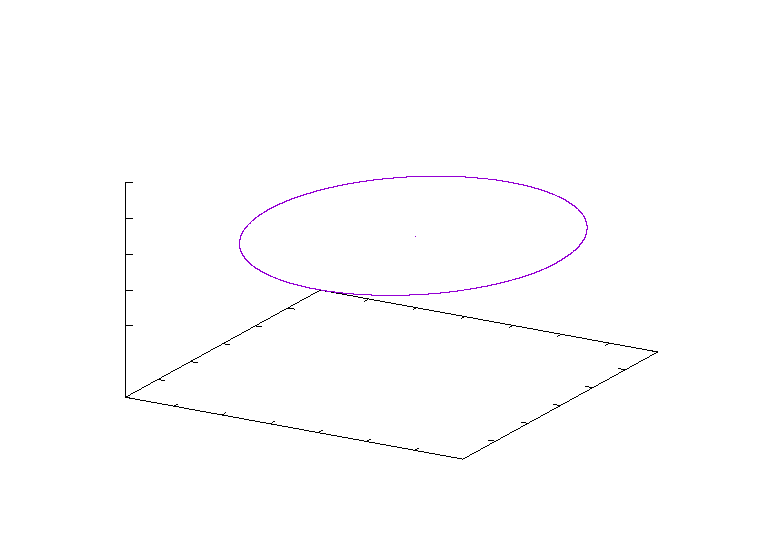
\includegraphics[width={360.00bp},height={252.00bp}]{plot}}%
    \gplfronttext
  \end{picture}%
\endgroup

\end{tiny}

\end{document}
